\documentclass[tikz,border=5pt]{standalone}
\usepackage[dvipsnames]{xcolor}
\usepackage{tikz}
\usetikzlibrary{arrows.meta,calc,fit,positioning,backgrounds,shapes.geometric}

\tikzset{
  component/.style={
    rectangle,
    draw=blue!50!black,
    fill=blue!12,
    rounded corners=2pt,
    minimum width=20mm,
    minimum height=20mm,
    inner sep=0pt
  },
  port/.style={
    rectangle,
    draw=black,
    fill=white,
    minimum width=7.5mm,
    minimum height=7.5mm,
    inner sep=0pt,
    font=\bfseries\small
  },
  inactiveport/.style={
    port,
    fill=gray!10,
    draw=gray!65,
    dashed,
    text=gray!70!black
  },
  connection/.style={
    very thick,
    ->,
    >=Latex
  },
  directfeedthrough/.style={
    ->,
    thick,
    dashed,
    red!75!black
  }
}

\newcommand{\arrowlegend}[1]{%
  \begin{scope}[shift={#1}]
    \draw[->, dashed, thick, red!75!black] (0,0) -- (0.7,0);
    \node[anchor=west, font=\small] at (0.75,0) {direct feedthrough};
    \draw[->, thick, black] (3.8,0) -- (4.5,0);
    \node[anchor=west, font=\small] at (4.55,0) {connection};
  \end{scope}%
}

\begin{document}
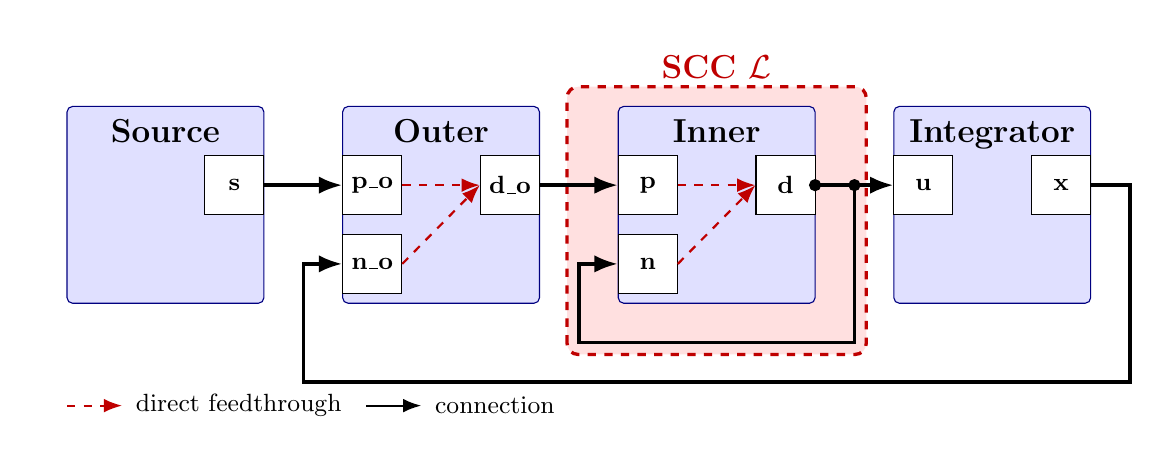
\begin{tikzpicture}[>=Latex]
  % Force identical bounding box across all four panels
  \useasboundingbox (-0.5, -1.5) rectangle (13.5, 3.5);
  %\draw[help lines, step=0.5] (-0.5,-1.5) grid (13.5,3.5);

  % Draw SCC boundary
  \draw[very thick, red!75!black, fill=red!12, rounded corners, dashed] (6.35, -0.65) rectangle (10.15, 2.75);
  \node[text=red!75!black] at (8.25, 3) {\large\bfseries SCC $\mathcal{L}$};

  % Source Component
  \begin{scope}[shift={(0,0)}]
    \draw[component] (0,0) rectangle (2.5,2.5);
    \node[anchor=north, font=\large\bfseries] at (1.25,2.45) {Source};
    \node[port] (A-y) at (2.125,1.5) {s};
  \end{scope}

  % Outer Subtractor
  \begin{scope}[shift={(3.5,0)}]
    \draw[component] (0,0) rectangle (2.5,2.5);
    \node[anchor=north, font=\large\bfseries] at (1.25,2.45) {Outer};
    \node[port] (B-pos) at (0.375,1.5) {p\_o};
    \node[port] (B-neg) at (0.375,0.5) {n\_o};
    \node[port] (B-y1) at (2.125,1.5) {d\_o};
    \draw[directfeedthrough] (B-pos) -- (B-y1);
    \draw[directfeedthrough] (B-neg.east) -- (B-y1.west);
  \end{scope}

  % Inner Subtractor
  \begin{scope}[shift={(7,0)}]
    \draw[component] (0,0) rectangle (2.5,2.5);
    \node[anchor=north, font=\large\bfseries] at (1.25,2.45) {Inner};
    \node[port] (C-pos) at (0.375,1.5) {p};
    \node[port] (C-neg) at (0.375,0.5) {n};
    \node[port] (C-y1) at (2.125,1.5) {d};
    \draw[directfeedthrough] (C-neg.east) -- (C-y1.west);
    \draw[directfeedthrough] (C-pos.east) -- (C-y1.west);
  \end{scope}

  % Integrator
  \begin{scope}[shift={(10.5,0)}]
    \draw[component] (0,0) rectangle (2.5,2.5);
    \node[anchor=north, font=\large\bfseries] at (1.25,2.45) {Integrator};
    \node[port] (D-u1) at (0.375,1.5) {u};
    \node[port] (D-y1) at (2.125,1.5) {x};
  \end{scope}

  \draw[connection] (A-y) -- (B-pos);
  \draw[connection] (B-y1) -- (C-pos);
  \draw[connection] (C-y1) -- (D-u1);
  \draw[connection] (C-y1) --++(0.375+0.5,0) --++(0,-2) --++(-3.5,0) --++(0,1) -- (C-neg);
  \draw[connection] (D-y1) --++(0.375+0.5,0) --++(0,-2.5) --++(-10.5,0) --++(0,1.5) -- (B-neg);

  \draw[black, fill=black] ({10}, {1.5}) circle (2pt);
  \draw[black, fill=black] ({9.5}, {1.5}) circle (2pt);




  \arrowlegend{(0, -1.3)}
\end{tikzpicture}
\end{document}